 %% Copyright (C) 2011, Andrea Cimino, All Rights Reserved. 
 %% This file is distributed under the terms of the Creative Common
 %% Licence Non-Commercial Share-Alike license

%% 11 Gennaio 2011

 %% Useful stuff for separate compilation.
\ifx\ismaindoc\undefined
\providecommand{\inbpdocument}{
 \documentclass[11pt,a4paper,twoside,titlepage]{scrbook}
%%%%%%%%%%%%%%%%%%%%%%%%%%%%%%%%
%%%%%%%%%%% PACKAGES %%%%%%%%%%%
%%%%%%%%%%%%%%%%%%%%%%%%%%%%%%%%
% encoding
\usepackage[utf8x]{inputenc}
\usepackage[italian]{babel} % babel (suddivisione parole in sillabe)

\usepackage{amsfonts} % matematica
\usepackage{amsmath} % matematica
\usepackage{amssymb} % simboli vari
\usepackage{calrsfs}
\usepackage{caption}
\usepackage{enumerate}
\usepackage{extarrows} % matematica
\usepackage{keyval}
\usepackage{manfnt} % Simboli curva
\usepackage{mathtools} % matematica
\usepackage{multirow} 
\usepackage[usenames]{color} % colori con nome
\usepackage[pdftex]{graphicx}
\usepackage{epstopdf} % gestione file EPS
\usepackage{wrapfig} % per figure circondate da testo
\usepackage{framed}	% teoremi framed
\usepackage{fancyhdr} % header buffi
\usepackage[T1]{fontenc} % gestione hbox e vbox
\usepackage[a4paper]{geometry}
\usepackage{microtype} % gestione hbox e vbox
\usepackage[thref, amsthm, amsmath, framed]{ntheorem} % teoremi (avanzata)
%% \usepackage{prooftree} % gestione prof-tree
\usepackage{rotating}
\usepackage{stmaryrd}
\usepackage{subfig}
\usepackage{syntax} % syntattic stuff
\usepackage{txfonts}
\usepackage{verbatim} % migliorie al verbatim
\usepackage{hyperref}
%% \usepackage{qtree}
\usepackage{fancyvrb}
\usepackage{listings}
\usepackage{cancel}
\usepackage{tikz}
\usepackage{cclicenses}

\usepackage{bbding} %% Icons

%%%%%%%%%%%%%%%%%%%%%%%%%%%%%%%%
%%%%%%%%%%% GEOMETRY %%%%%%%%%%%
%%%%%%%%%%%%%%%%%%%%%%%%%%%%%%%%
\geometry{verbose,tmargin=2cm,bmargin=2.5cm,lmargin=2.5cm,rmargin=2cm}
\parindent0ex %% Remove paragraph indenting

%%%%%%%%%%%%%%%%%%%%%%%%%%%%%%%%
%%%%%%%%%%% CODE ENV %%%%%%%%%%%
%%%%%%%%%%%%%%%%%%%%%%%%%%%%%%%%
% codice
\newcounter{count}
\setcounter{count}{0}
\newenvironment{code}[1]
{
\color{lightgray}\hrulefill\color{code}
\stepcounter{count} {\bf\small Listato di codice \arabic{count}: {#1} }
\verbatim
}
{
\endverbatim
\color{lightgray}\hrulefill
\color{black}
\\
}

% codice semplice
\newenvironment{simplecode}
{
\color{code} \tt
}
{
\rm
}

 % Notation issues
\input{macros}

\makeatletter
\g@addto@macro\@verbatim\footnotesize
\makeatother



%%%%%%%%%%%%%%%%%%%%%%%%%%%%%%%%
%%%%%%%% THEOREMS FORMAT %%%%%%%
%%%%%%%%%%%%%%%%%%%%%%%%%%%%%%%%
% shaded theorems and proofs command
\definecolor{lightgray}{RGB}{230,230,230}
\def\theoremframecommand{\colorbox{lightgray}}

%%% theorems
\theoremstyle{break}
\theoremheaderfont{\normalfont\bfseries}
\theorembodyfont{\itshape}
\theoremsymbol{\ensuremath{\diamondsuit}}
\theoremseparator{\newline}
\newshadedtheorem{theo}{\includegraphics[scale=0.11]{imgs/book.png}
Teorema}[chapter]

%%% propositions
\theoremstyle{break}
\theoremheaderfont{\normalfont\bfseries}
\theorembodyfont{\itshape}
\theoremsymbol{\ensuremath{\diamondsuit}}
\theoremseparator{\newline}
\newshadedtheorem{proposition}{Proposizione}[chapter]

%%% exercises
\theoremstyle{break}
\theoremheaderfont{\normalfont\bfseries}
\theorembodyfont{\itshape}
\theoremsymbol{\ensuremath{\diamondsuit}}
\theoremseparator{\newline}
\newshadedtheorem{exercise}{Esercizio}[chapter]

%%% propositions
\theoremstyle{break}
\theoremheaderfont{\normalfont\bfseries}
\theorembodyfont{\itshape}
\theoremsymbol{\ensuremath{\diamondsuit}}
\theoremseparator{\newline}
\newshadedtheorem{property}{\PencilRightDown $\; $ Propriet\`a}[chapter]
%%% lemmas
\theoremstyle{break}
\theoremheaderfont{\normalfont\bfseries}
\theorembodyfont{\itshape}
\theoremsymbol{\ensuremath{\diamondsuit}}
\theoremseparator{\newline}
\newshadedtheorem{lemma}[theo]{Lemma}

%%% definitions
\theoremstyle{break}
\theoremsymbol{\ensuremath{\clubsuit}}
\theoremseparator{\newline}
\newshadedtheorem{defn}[theo]{Definizione}

%%% examples
\theoremstyle{break}
\theorembodyfont{\itshape}
\theoremsymbol{\ensuremath{\ast}}
\theoremseparator{\newline}
\newshadedtheorem{example}[theo]{Esempio}

%%% observations
\theoremstyle{break}
\theorembodyfont{\itshape}
\theoremsymbol{\ensuremath{\ast}}
\theoremseparator{\newline}
\newshadedtheorem{observation}[theo]{
\includegraphics[scale=0.06]{imgs/lens.png}
Osservazione
}

%%% notations
\newtheorem*{notaz}{Notazione}

%%% proofs
\newenvironment{thproof}
{
\vskip 0.03cm
\begin{small}
\textit{Dimostrazione. }
\color{code}
}
{
\color{black}
\end{small}
$ \square $
\vskip 0.2cm
}

%Notes
\newenvironment{notes}{%
  \def\FrameCommand{\colorbox{yellow}}%
  \MakeFramed {\FrameRestore}
\includegraphics[scale=0.02]{imgs/bulb.png}
 \textbf{Nota} \\
 }%
{\endMakeFramed}

%Work in progress
\newenvironment{workinprogress}{%
  \def\FrameCommand{\colorbox{pink}}%
 
 \MakeFramed 
 {\FrameRestore}
\lhdbend  \textbf{Work in progress} \\
\\
 }%
{\endMakeFramed}

%Openquestion
\newenvironment{openquestion}{%
  \def\FrameCommand{\colorbox{pink}}%
  \MakeFramed {\FrameRestore}
 \textbf{Domanda aperta} \\
 }%
{\endMakeFramed}

%TODO
\newenvironment{todo}{%
  \def\FrameCommand{\colorbox{pink}}%
  \MakeFramed {\FrameRestore}
 \textbf{TODO} \\
 }%
{\endMakeFramed}

%%%%%%%%%%%%%%%%%%%%%%%%%%%%%%%%
%%%%%%%%%%%% HEADER %%%%%%%%%%%%
%%%%%%%%%%%%%%%%%%%%%%%%%%%%%%%%
\pagestyle{fancy}
% i comandi seguenti impediscono la scrittura in maiuscolo
% dei nomi dei capitoli e dei paragrafi nelle intestazioni
\renewcommand{\chaptermark}[1]{\markboth{#1}{}}
\renewcommand{\sectionmark}[1]{\markright{\thesection\ #1}}
\fancyhf{} % rimuove l'attuale contenuto dell'intestazione
% e del pi\`e di pagina
\fancyhead[LE,RO]{\bfseries\thepage}
\fancyhead[LO]{\bfseries\rightmark}
\fancyhead[RE]{\bfseries\leftmark}
\renewcommand{\headrulewidth}{0.5pt}
\renewcommand{\footrulewidth}{0pt}
\addtolength{\headheight}{0.5pt} % riserva spazio per la linea
\fancypagestyle{plain}{%
\fancyhead{} % ignora, nello stile plain, le intestazioni
\renewcommand{\headrulewidth}{0pt} % e la linea
}


%%%%%%%%%%%%%%%%%%%%%%%%%%%%%%%%
%%%%%%%%%%%% COLORS %%%%%%%%%%%%
%%%%%%%%%%%%%%%%%%%%%%%%%%%%%%%%
\definecolor{code}{gray}{0.3}


%%%%%%%%%%%%%%%%%%%%%%%%%%%%%%%%
%%%%%%%%%%%% NUMBERS %%%%%%%%%%%
%%%%%%%%%%%%%%%%%%%%%%%%%%%%%%%%
\setcounter{tocdepth}{3}
\setcounter{secnumdepth}{3}


%%%%%%%%%%%%%%%%%%%%%%%%%%%%%%%%
%%%%%%%%%%% DOC DATA %%%%%%%%%%%
%%%%%%%%%%%%%%%%%%%%%%%%%%%%%%%%
\title{Appunti di MNO}
\author{Gruppo Informatici Rampanti}
\date{ott 2010 - mag 2011}

\pdfinfo{%
  /Title    (Appunti di MNO)
  /Author   (Andrea Cimino e Lorenzo Muti)
  /Creator  (Andrea Cimino)
  /Producer (Lorenzo Muti)
  /Subject  (MNO)
  /Keywords (MNO)
}


%%%%%%%%%%%%%%%%%%%%%%%%%%%%%%%%
%%%%%%%%%%%%% UTILS %%%%%%%%%%%%
%%%%%%%%%%%%%%%%%%%%%%%%%%%%%%%%
% binary symbols
\newcommand{\modder}{\vdash _{R}}

% vertical gaps
\newcommand{\askip}{\vspace{0.5cm}}
\newcommand{\bskip}{\vspace{1.0cm}}

% various symbols
\newcommand{\qedhere}{\ensuremath{\Box}}
\newcommand{\qed}{\hfill \ensuremath{\Box}}

% substitution
\newcommand{\subst}[2]{^{#1} / _{#2}}

% denotational semantics function names
\newcommand{\bbracket}[1]{\left\llbracket #1 \right\rrbracket}

\newcommand{\aexpr}{\mathcal{A}}
\newcommand{\bexpr}{\mathcal{B}}
\newcommand{\cexpr}{\mathcal{C}}
\newcommand{\Aexpr}[1]{\mathcal{A} \bbracket{#1}}
\newcommand{\Bexpr}[1]{\mathcal{B} \bbracket{#1}}
\newcommand{\Cexpr}[1]{\mathcal{C} \bbracket{#1}}

\newcommand{\semdomset}[1]{(V_{#1})_{\bot}}

% semantic evaluations
\newcommand{\opereval}[3]{\left\langle #1, #2 \right\rangle \rightarrow #3}
\newcommand{\denaeval}[3]{\Aexpr{#1} #2 = #3}
\newcommand{\denbeval}[3]{\Bexpr{#1} #2 = #3}
\newcommand{\denceval}[3]{\Cexpr{#1} #2 = #3}

% rotated sqsubseteqs
\newcommand{\upsqsubseteq}{ $\begin{rotate}{90} $\sqsubseteq$ \end{rotate}$ }
\newcommand{\downsqsubseteq}{ $\begin{rotate}{270} $\sqsubseteq$ \end{rotate}$ }

% Space after paragraph declaration
\makeatletter
\renewcommand\paragraph{\@startsection{paragraph}{4}{\z@}%
  {-3.25ex\@plus -1ex \@minus -.2ex}%
  {1.5ex \@plus .2ex}%
  {\normalfont\normalsize\bfseries}}
\makeatother

\begin{document}
}
\providecommand{\outbpdocument}{\end{document}}
\else
\providecommand{\inbpdocument}{}
\providecommand{\outbpdocument}{}
\fi




 \inbpdocument

\chapter{Ottimizzazione non vincolata}
\label{chap:ottimizzazione-non-vincolata}
 Il problema che affronteremo in
questo capitolo è quello gi\`a enunciato nel Capitolo
\ref{chap:ottimizzazioni-definizioni}, ovvero quello
dell'ottimizzazione \emph{non vincolata}, nel quale si cerca il minimo
di una funzione in tutto lo spazio $\mathbb{R}^n$:

$$ \min\{ f(x): x \in \mathbb{R}^n \} \quad  f: \mathbb{R}^n: \mathbb{R}$$
Abbiamo gi\`a visto che in questo tipo di problemi il minimo si trova
necessariamente in un punto $\overline{x}$ stazionario, ovvero
$$\overline{x}~ \text{punto di minimo}\quad \Longrightarrow \quad \nabla f(\overline{x})=0$$

Nel caso che la funzione sia convessa, questa \`e condizione anche
sufficiente. Nel caso che la funzione sia quadratica, il
soddisfacimento della condizione si riconduce alla risoluzione di un
sistema lineare. Altrimenti, in generale il problema che si forma \`e
non--lineare, e lo possiamo risolvere ad esempio con il metodo
Newton--Raphson visto nella Sezione
\ref{section:metodo-newton-raphson}. In questo capitolo vedremo alcuni
metodi iterativi (di cui uno basato su Newton-Raphson) per risolvere
il problema nel caso che $f$ sia non lineare.

Ma guardiamo innanzi tutto degli esempi di questi problemi.

\begin{example}
\label{esempio-prog-nv} Vediamo un semplice problema di ottimizzazione
non vincolata. Abbiamo un piano diviso da una retta (in 2
semipiani). In questi piani un oggetto si muove attraverso due mezzi
$M_1$ e $M_2$ (es. acqua, aria) che hanno velocit\`a di percorrenza
rispettivamente $v_1, v_2$. L'oggetto deve muoversi da un punto $p \in
M_1$ a $q \in M_2$ minimizzando il tempo di percorrenza.\\ Per
semplificare il modello, si prende l'asse $x$ passante per $p$ e
scegliamo un'unit\`a di misura tale che sia $p=(-1,0)$.

\centerline{\includegraphics[width=0.60\textwidth]{imgs/esempio-prog-nv.png}}

All'interno dello stesso mezzo, il percorso pi\`u breve tra due punti \`e
ovviamente la retta. Il percorso sar\`a dunque determinato dal parametro
$x$, ordinata del punto in cui il percorso passa da $M_1$ a $M_2$, e
sar\`a composto da due segmenti che uniscono i punti $p=(-1,0),
x'=(0,x), q=(q_1, q_2)$.\\ I due segmenti sono lunghi rispettivamente
$\sqrt{1+x^2}$ e $\sqrt{q_1^2 + (q_2 - x)^2}$.\\ La funzione che
calcola il tempo di percorrenza, da minimizzare, \`e la seguente:
$$f(x) =  \frac{\sqrt{1+x^2}}{v_1} + \frac{\sqrt{q_1^2 + (q_2 - x)^2}}{v_2}$$
Dobbiamo risolvere il problema di ottimizzazione senza vincoli:
$$ \min\{f(x):\; x \in \mathbb{R}\}$$
Cerchiamo i punti in cui il gradiente della funzione si annulla. Dato
che la funzione \`e a una variabile, il gradiente \`e la derivata:
$$\nabla f(x)= f'(x)=0$$

$$f'(x) = \frac{1}{v_1} \frac{2x}{2 \cdot \sqrt{1+x^2}} + \frac{1}{v_2} \frac{2x - 2q_2}{2\sqrt{q_1^2 + (q_2 - x)^2}} = \frac{x}{v_1\sqrt{1+x^2}} - \frac{{q_2 - x}}{v_2 \sqrt{q_1^{2} + (q_2 -x)^2}}
$$
Notiamo che i denominatori non si annullano mai e risolviamo $f'(x) =
0$.
$$ v_2 x \sqrt{q_1^2 + (q_2 -x)^2} - v_1(q_2 -x)\sqrt{1+x^2}=0$$ \\
Abbiamo ottenuto una funzione non lineare che da il punto di
stazionariet\`a. Inoltre la funzione \`e convessa, quindi in questo caso
la condizione $f'(x)=0$ \`e necessaria e sufficiente perch\'e la funziona
sia minima. \\ \textbf{Esercizio}: dimostra che $f'(x)$ \`e convessa.\\
Riscriviamo l'equazione come:

\begin{equation}
\label{eq:esempio-ottimizzazione-nv-1} \frac{x}{\sqrt{1+x^2}} \cdot
\frac{\sqrt{q_1^2 + (q_2-x)^2}}{q_2 -x} =\frac{v_1}{v_2}
\end{equation}

Facciamo intanto un'osservazione. Dato che le velocit\`a sono positive,
\`e
$$\frac{v_1}{v_2} > 0 \quad \Longrightarrow \quad \frac{x}{q_2-x} \geq 0 \quad \Longrightarrow \quad 0 \leq x \leq q_2$$
Abbiamo ristretto lo spazio in cui cercare la soluzione ottimale.

\centerline{\includegraphics[width=0.50\textwidth]{imgs/esempio-prog-nv2.png}}

Diamo dei nomi ai punti come nella figura sopra e riscriviamo la
\ref{eq:esempio-ottimizzazione-nv-1} rinominando i membri delle
frazioni come:

$$\frac{\overline{AB}}{\overline{PA}} \cdot \frac{\overline{AQ}}{\overline{QC}} = \frac{v_1}{v_2}$$

Guardando la figura, si noti come
$$\frac{\overline{AB}}{\overline{PA}} = \sin \theta_1, \quad \frac{\overline{AQ}}{\overline{QC}} = \frac{1}{\sin \theta_2}$$
Abbiamo ottenuto che la durata di percorrenza $f(x)$ si minimizza
quando
$$ \frac{\sin \theta_1}{\sin \theta_2} = \frac{v_1}{v_2}$$
(Tra l'altro, questa \`e la legge della rifrazione di
Snell--Cartesio.)\\ \`E un'equazione non lineare ad una variabile che si
può risolvere con i classici metodi del calcolo numerico, ad esempio
applicando il Metodo delle Tangenti nell'intervallo $[0, q_2]$.
\end{example}

\begin{example} Nell'esempio \ref{esempio-prog-nv} la funzione che
abbiamo ottenuto per la ricerca del punto stazionario era ad una
variabile. Complichiamo il problema in modo da ottenere una funzione a
due variabili.

\centerline{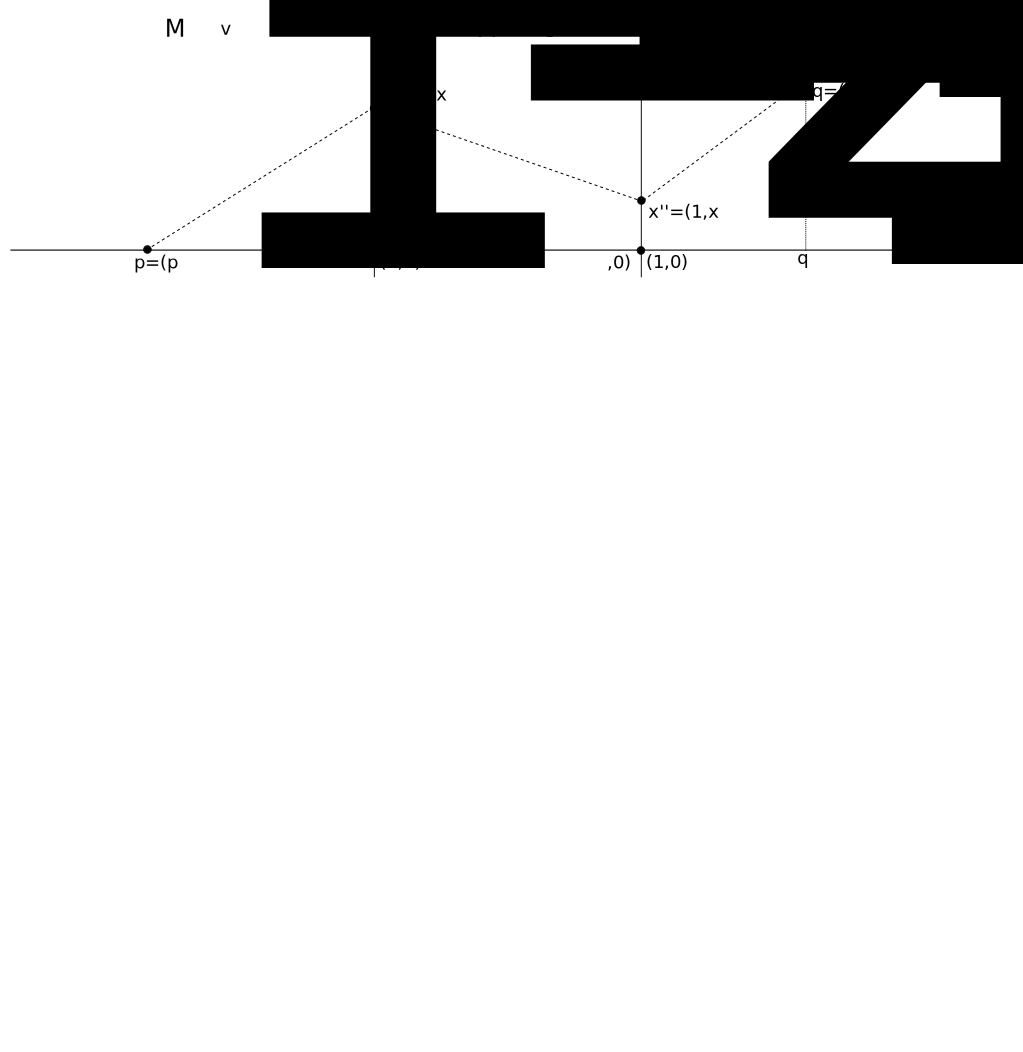
\includegraphics[width=0.80\textwidth]{imgs/esempio-prog-nv-2var.png}}

Il problema \`e simile ma invece di due, i mezzi sono tre: $M_1, M_2,
M_3$, divisi da due rette parallele. Per semplificare i conti,
posizioniamo gli assi in modo che le rette di separazione dei piani
siano verticali e il punto $p$ di partenza sia sull'asse delle
ascisse, e scegliamo un'unit\`a di misura tale che il semipiano $M_2$
sia largo $1$.\\ Stavolta per individuare un tragitto sono necessari i
due parametri $x_1$ e $x_2$, ovvero il valore dell'ordinata dei punti
$x'$ e $x''$ in cui il tragitto passa da un mezzo all'altro.\\ La
funzione che calcola la velocit\`a di percorrenza \`e $$f(x_1, x_2) =
\frac{\sqrt{p_1^2 + x_1^2}}{v_1} + \frac{\sqrt{1+ (x_2 - x_1)^2}}{v_2}
+ \frac{\sqrt{(q_1 -1)^2 + (q_2 - x_2)^2}}{v_3}$$ Abbiamo un problema
di minimizzazione, anche questo non vincolato, in 2 variabili: $$
\min\{f(x):\; x \in \mathbb{R}^2\}$$ $f(x)$ \`e convessa, quindi
$\nabla(x) = 0$ \`e condizione necessaria e sufficiente per la
minimalit\`a di $f(x)$.\\ \textbf{Esercizio}: dimostrare che $f(x)$ \`e
convessa. \\ Cerchiamo dove $$\nabla f(x) = 0$$ Stavolta $\nabla f(x)$
\`e un vettore a due dimensioni. Vediamone le componenti, che si devono
annullare:\\
$$\frac{\partial f}{x_1}(x_1,x_2) =  \frac{x_1}{v_1 \sqrt{p_1^2+ x_1^2}} - \frac{x_2 - x_1}{v_2 \sqrt{1+(x_2 - x_1)^2}} = 0$$
$$\frac{\partial f}{x_2}(x_1,x_2) =  \frac{x_2-x_1}{v_2 \sqrt{1+( x_2-x_1)^2)}} - \frac{q_2 -x_2}{v_3  \sqrt{(q_1-1)^2 + (q_2 -x_2)^2}} = 0$$
Questo \`e un sistema non lineare di due equazioni in due
incognite. Condizione necessaria e sufficiente perch\'e la soluzione
$x=(x_1,x_2)$ sia minima \`e che il sistema sia soddisfatto.

Questo particolare sistema si può risolvere con i metodi classici del
calcolo numerico, ad esempio il metodo delle tangenti (detto anche
Newton--Raphson), cercando sia $x_1$ che $x_2$ nell'intervallo
$[0,q_2]$).
\end{example}

\section{Metodi risolutivi per i problemi di ottimizzazione non
vincolata} Abbiamo visto negli esempi dei problemi che si riducono
alla risoluzione di un sistema non vincolato di equazioni non lineari,
e abbiamo accennato al fatto che questi sistemi, in alcuni casi,
possono essere risolti con i metodi del calcolo numerico (es. Metodo
delle tangenti, delle secanti o di bisezione). Va notato però che
questi metodi hanno bisogno come dato di input dell'intervallo entro
cui cercare la soluzione, e della garanzia che questo intervallo
contenga una sola soluzione. Sebbene questo sia possibile nei due
esempi presi in considerazione, non \`e possibile in generale.

Guardiamo quindi a dei metodi iterativi in grado di risolvere un
generico problema di ottimizzazione non vincolata. Il problema si pone
come
$$ (P) \quad \min\{f(x)\; : \; x \in \mathbb{R}^n\} \quad f: \mathbb{R}^n  \rightarrow \mathbb{R} \text{ differenziabile}$$
I metodi che vedremo sono tutti di natura iterativa, genereranno
dunque una successione di valori $ x^0, x^1, \ldots, x^k$. Quello che
cerchiamo, come sempre, sono i punti stazionari $x^{*}$, ovvero tali
che
$$\nabla f(x^{*}) = 0$$

Se la funzione \`e convessa, come sappiamo $\nabla f(x^{*}) = 0$ \`e
condizione sufficiente, oltre che necessaria, perch\'e $x$ sia punto di
minimo, dunque nelle funzioni convesse i punti stazionari sono anche
punti di minimo. Altrimenti, se $f$ non \`e convessa,$\nabla f(x^{*}) =
0$ \`e comunque condizione necessaria per essere punto di minimo, quindi
siamo comunque interessati a cercare i punti in cui il gradiente si
annulla perch\'e candidati ad essere minimi.

L'unica ipotesi di cui abbiamo bisogno per questo tipo di metodi \`e che
$f$ sia differenziabile (ma in alcuni metodi porremo il vincolo che
$f$ sia differenziabile con continuit\`a, cio\`e che il suo gradiente
$\nabla f$ sia una funzione continua, oppure che sia differenziabile
due volte).

In questi metodi, trovare $\overline{k}$ t.c. $\nabla
f(x^{\overline{k}}) = 0$ può essere un processo infinito. Non potendo
garantire la finitezza, ciò che chiediamo ai nostri metodi \`e la
convergenza, che può essere definita in diversi modi:

\begin{enumerate}
\item Il limite esiste ed \`e un punto stazionario: $$\exists \lim_{k
\to \infty} x^{k} = x^{*} \quad \text{e} \quad \nabla f(x^{*}) = 0$$
\item Definizione pi\`u debole: se la successione converge, allora
converge al punto stazionario (ma non \`e detto che converga!). Quindi
tutti i punti di accumulazione di $\{x^k\}$ sono stazionari (ma non \`e
detto che ne esistano): $$\lim_{k \to \infty} x^{k} = x^{*} \quad
\Longrightarrow \quad \nabla f(x^{*}) = 0$$
\item Definizione ancora pi\`u debole: almeno un punto di accumulazione
della successione $\{x^k\}$ \`e stazionario.
\end{enumerate}

Tra i metodi iterativi, daremo particolare attenzione ai Metodi di
discesa:
\begin{defn}[Metodo di discesa] Quei metodi iterativi tali che ad ogni
iterazione, il valore della funzione obiettivo decresce: $$ f(x^0) >
f(x^1) > f(x^2) > \ldots > f(x^k) > \ldots $$
\end{defn}

In particolare, si dice Metodo di discesa \emph{non
monotòna}\footnote{Utilizzeremo raramente questa definizione.} se:
\begin{defn}[Metodo di discesa non monotòna] Dopo $n$ iterazioni ($n$
fissato), il valore della funzione obiettivo decresce:
$$ \exists ~ n \in \mathbb{N} \quad \text{t.c.} \quad \forall k \quad f(x^k) > f(x^{k+n}) $$
\end{defn}

\subsection{Ricerca monodimensionale} Nei metodi di ricerca
monodimensionale (line search), se nella $k$-esima iterazione abbiamo
ottenuto il punto $x^k$, otteniamo il punto $x^{k+1}$ muovendoci dal
punto $x^k$ lungo una direzione $d^k$ di un passo lungo $t_k$
(direzione e ampiezza del passo sono scelti ad ogni iterazione). Si
chiama \emph{monodimensionale} proprio perch\'e l'ampiezza del passo
$t_k$ \`e scelta su un'unica dimensione (lungo $d^k$). Tipicamente si
sceglie $d^k$ t.c. $\Vert d^k \Vert = 1$.

\centerline{\includegraphics[width=0.40\textwidth]{imgs/ricerca-monodimensionale-passo.png}}

In formule:
$$ x^{k+1} = x^{k} + t_k d^{k} \quad t_k \in \mathbb{R}^{n} \quad
  \begin{array}{l} t_k \in \mathbb{R}\text{ passo di spostamento} \\
d^{k} \in \mathbb{R}^n \text{ direzione}
  \end{array}
$$
%$$ t_k \in argmin \{ f(x^{k}+td^{k}) : t \geq 0  \}$$

\begin{notes} Anche l'algoritmo del simplesso per la programmazione
lineare vincolata \`e un metodo di line search, visto che da un vertice
ci si muove lungo una direzione (cio\`e lungo il bordo dei vincoli) per
giungere ad un altro vertice.
\end{notes}

I metodi di ricerca monodimensionale si differenziano tra loro
per il modo in cui, ad ogni passo, viene scelta la
direzione $d$ e l'ampiezza $t$ del passo successivo.

Vediamo innanzi tutto come ottenere un metodo di discesa. Supponiamo,
ad un generico passo, di aver ottenuto $ \overline{x} \in
\mathbb{R}^{n}$ (non stazionario, cio\`e tale che $\nabla
f(\overline{x}) \neq 0$, altrimenti abbiamo gi\`a la soluzione).

Dato che $f$ \`e differenziabile, abbiamo lo sviluppo di Taylor:
$$f(\overline{x} +t \cdot d) -f(\overline{x}) = t \cdot \nabla f(\overline{x})^{T} \cdot d + r(td)$$

Dove $r(td)$ \`e un resto tale che $\frac{r(td)}{t}$ va a $0$ per $||t|| \longrightarrow 0$. Inoltre
sappiamo che

$$ \lim_{t \to 0} \frac{f(\overline{x}+td)- f(\overline{x})}{t} = \nabla f(\overline{x})^{T} \cdot d $$

Da questa equazione si ricava che, se scegliamo la direzione $d$ in
modo che sia $\nabla f(\overline{x})^{T} \cdot d < 0$, in un intorno
di $t=0$ sufficientemente piccolo l'argomento del limite deve essere
negativo:

$$\exists ~ \varepsilon ~ \text{t.c.}~ \forall ~ t \in [0,\varepsilon] \quad \frac{f(\overline{x}+td)- f(\overline{x})}{t} < 0$$

ma dato che $t>0$, deve necessariamente essere $f(\overline{x}+td)-
f(\overline{x}) < 0$ e dunque $f(\overline{x}+td) < f(\overline{x})$,
che \`e proprio ciò che cercavamo.

Ricapitolando:
\begin{property}
\label{prop:metodo-discesa-gradiente-direzione} se si sceglie
$$d \quad \text{t.c.} \quad \nabla f(\overline{x})^{T} \cdot d < 0 \quad \text{e} \quad  t \in (0, \varepsilon) \text{ con }\varepsilon\text{ sufficientemente piccolo} \quad \Longrightarrow \quad \text{il passo } x^{k} + t_k d^{k} \text{ \`e di discesa} $$
\end{property}
\subsection{La massima decrescita}
\label{subsection:massima-decrescita} Naturalmente, il nostro
interesse \`e che il metodo non solo sia di discesa, ma che discenda pi\`u
velocemente possibile. Cerchiamo quindi di prendere $d$ in modo che il
prodotto non solo sia negativo, ma il pi\`u negativo possibile. Per
andare incontro a questa esigenza, si forma un altro problema:
\begin{equation}
\label{prob:pa} (Pa) \quad \min \{ \nabla f(\overline{x})^{T}d :
||d||_2 = 1 \}
\end{equation}

\begin{notes} La norma di $d$ deve essere limitata, ad es. con
$||d||_2 = 1$, altrimenti supponiamo di trovare una direzione
$$ \overline{d} = dt \quad \text{t.c.} \quad \nabla f(\overline{x})^{T} \overline{d} < 0 \quad \Longrightarrow \quad\nabla f(\overline{x})^{T} \overline{d} = \nabla f(\overline{x})(td) = t(\nabla f(\overline{x})^{T}d)$$
Ma se mandiamo $t$ a $+\infty$:
$$t(\nabla f(\overline{x})^{T}d) \longrightarrow_{t \to +\infty} - \infty$$
E il problema risulta inferiormente illimitato.
\end{notes}

Il problema di ottimizzazione \ref{prob:pa} lo sappiamo risolvere per
via teorica. Si ricorda che il prodotto scalare tra due vettori $a$ e
$b$ si calcola come

\centerline{\includegraphics[width=0.20\textwidth]{imgs/a-b-theta.png}}

$$a^{T}b = ||a||_{2} ||b||_2 \cos \theta$$
Quindi tenendo conto che $||d||_2 = 1$, il prodotto scalare
$f(\overline{x})^{T}d$ si calcola come
$$\nabla f(\overline{x})^{T} d =  || \nabla f(\overline{x})||_{2} \cos \theta$$
In cui $\overline{x}$ e $f$ sono fissati, quindi $f(\overline{x})$ \`e
un numero fissato nel nostro problema.

Quindi il problema si può riscrivere come:
$$ \min \{ \nabla f(\overline{x})^{T}d ~ : \Vert d \Vert = 1 \} ~ =  ~ \Vert\nabla f(\overline{x})\Vert_{2} \cdot \min\{ \cos \theta ~ : \Vert d \Vert_{2}=1 \}$$
Notare che $d$ sembra scomparire nella formula, in realt\`a $\theta$
dipende da $d$ (e da $f(\overline{x})$ che \`e fisso per il problema).
Il minimo di questo problema si ottiene quando
$$ \cos \theta = -1 \quad \Longleftrightarrow \quad  \theta = \pi $$

Ma perch\'e questo angolo sia $\pi$, \`e necessario che si prenda $d$
nella direzione opposta rispetto al gradiente. Inoltre vogliamo $d$ di
norma unitaria, e per questo basta dividerlo per la norma del
gradiente.
$$\quad \Longleftrightarrow \quad d = \frac{- \nabla f(\overline{x})}{|| \nabla f(\overline{x})||_{2}}$$
In altre parole, sto chiedendo che $d$ sia il versore della direzione
opposta al gradiente.

Ancora una volta, il gradiente \`e la direzione di massima crescita,
quindi la massima decrescita \`e la direzione opposta al gradiente.

\section{Metodi del gradiente} Da quanto visto sopra, si deduce
facilmente un primo metodo di ricerca monodimensionale in cui la
direzione $d$ scelta ad ogni passo \`e l'opposto del gradiente:

$$ x^{k+1} = x^{k} + t_k \cdot d^k \quad \text{con} ~ d^{k} = - \nabla f(x^{k})$$
Ovvero
$$ x^{k+1} = x^{k} - t_k \cdot \nabla f(x^{k})$$

(Avremmo potuto prendere $d^k = - \frac{\nabla f(k^k)}{\Vert \nabla
f(x^k)\Vert_{2}}$, ma lasciamo perdere la divisione per la norma del
gradiente perch\'e la consideriamo ``inglobata'' nel passo di
spostamento.)

Per quanto riguarda la scelta del passo di spostamento $t_k$, la
scelta ideale \`e ovviamente di prenderlo esatto:
\begin{defn}[Metodo della Ricerca Esatta] Metodo nel quale la
lunghezza del passo si calcola con un nuovo problema di
ottimizzazione:
$$ t_k \in \text{ arg min } \{f(x^{k} - t_k \nabla f(x^{k})): \; t_k \geq 0 \}$$
Ovvero il passo \`e cercato lungo la semiretta in modo che minimizzi la
funzione obiettivo.
\end{defn}

\begin{defn}[Metodo del Gradiente Esatto]
\label{def:metodo-gradiente-esatto} Metodo del gradiente (ovvero tale
che $d^{k} = - \nabla f(x^{k})$) in cui si sceglie il passo col metodo
della ricerca esatta.

Sotto forma di algoritmo si può enunciare come segue:
\begin{enumerate}
 \item Poniamo $k=0$; Si sceglie un punto di partenza $x_0$;
 \item Se $\nabla f(x^{k})=0$, allora STOP: abbiamo trovato un punto
stazionario. \label{passo-algoritmo-gradiente-esatto-test-stop}
 % un label e' per sempre!
\item Si calcola la direzione come l'opposto del gradiente: $ d^k = - \nabla
 f(x^{k})$;\label{passo-algoritmo-gradiente-esatto-scelta-direzione}
 \item \label{passo-algoritmo-gradiente-esatto-scelta-passo}Si calcola
il passo con la ricerca esatta:
$$t_k \in argmin \{ f(x^{k} + t_k
\cdot d^k) \; : \; t_k \geq 0 \}$$
ovvero
$$t_k \in argmin \{ f(x^{k} - t_k
\cdot \nabla f(x^{k})) \; : \; t_k \geq 0 \}$$
 \item Ci si sposta al punto successivo: $x^{k+1} =x^{k} + t_k \cdot d^k = x^{k} - t_k \cdot
\nabla f(x^{k})$
 \item $k:=k+1$, ritornare al passo
\ref{passo-algoritmo-gradiente-esatto-test-stop}.
\end{enumerate}
\end{defn}

Come vedremo in seguito (\ref{critica-gradiente-esatto}), il passo
\ref{passo-algoritmo-gradiente-esatto-scelta-passo} impone la
soluzione di un problema di ottimizzazione esatta che, in generale, \`e
tutt'altro che banale, per questo vedremo altri metodi del gradiente
che non utilizzano la ricerca esatta ma scelgono il passo in maniera
pi\`u approssimata e meno costosa. Tuttavia per alcune funzioni
obiettivo particolari, ad es. le funzioni quadratiche, il calcolo
della ricerca esatta \`e possibile e facilmente risolvibile, perch\'e la
funzione da minimizzare $f(x^{k} - t_k \nabla f(x^{k}))$ \`e una
parabola con il vertice verso l'alto, della quale \`e facile calcolare
esattamente il minimo.

\subsection{Propriet\`a del Metodo del Gradiente Esatto} Abbiamo
intenzione di dimostrare tre propriet\`a del Metodo del Gradiente
Esatto:
\begin{enumerate}
\item Il metodo del gradiente esatto \`e un metodo di discesa;
\item Due direzioni successive del metodo del gradiente esatto sono
tra loro ortogonali;
\item Il metodo converge.
\end{enumerate}

Per queste dimostrazioni, si introduce la seguente funzione:
$$\varphi(t) = f(x^{k} - t \nabla f(x^{k}))$$
Questa \`e la funzione $f$ calcolata lungo la semiretta nella quale
viene cercato il passo di spostamento, vista come funzione del passo
$t$. \`E la funzione di ricerca: durante la ricerca esatta si cerca il
minimo di $\varphi$. Si noti che \`e la composizione di due funzioni:
$$ t \xlongrightarrow{\theta} x^{k}-t\nabla f(x^{k}) \xlongrightarrow{f} f(x^{k} - t \nabla f(x^{k}))$$

La funzione $\theta: \mathbb{R} \rightarrow \mathbb{R}^{n}$ associa il
passo $t$ al punto trovato, mentre $f: \mathbb{R}^{n} \rightarrow
\mathbb{R}$ associa il punto trovato al valore della funzione
obiettivo. $\varphi$ si scrive come $ \varphi= f \circ \theta :
\mathbb{R} \rightarrow \mathbb{R}$.

$\theta$ si può vedere come un insieme $(\theta_{1}, \ldots,
\theta_{i}, \ldots, \theta_{n})$ di $n$ funzioni, una per ogni
componente, tali che $\theta_{i}: \mathbb{R} \rightarrow \mathbb{R}$
assume il valore dell'$i$-esima componente del vettore $x^{k}-t\nabla
f(x^{k}) = \theta(t)$. Quindi

$$ \theta = (\theta_{1}, \theta_{2}, \ldots, \theta_{n}) \qquad \theta(t) = x^{k}-t\nabla f(x^{k}) =  \left(\begin{matrix}\theta_{1}(t) \\\theta_{2}(t) \\ \vdots \\ \theta_{n}(t)\end{matrix}\right)$$

La funzione $\theta$ \`e derivabile, quindi ogni $\theta_i$ \`e
derivabile.
$$ \theta' = (\theta_1', \theta_2', \ldots, \theta_{n}' )$$

Si noti quindi che
$$
\left.\begin{matrix} f \text{ \`e differenziabile}\\ \theta_i \text{
sono derivabili} \\
\end{matrix}\right. ~ \Longrightarrow ~ \varphi = f \circ \theta
\text{ \`e derivabile}
$$

e la sua derivata \`e \footnote{ Usando il seguente teorema
  \begin{theo}
    \label{theo:derivata-funzioni-composte} Sia $\Theta:\mathbb{R}
\rightarrow \mathbb{R}^{n}$ derivabile in $\overline{t}\in \mathbb{R},
g: \mathbb{R}^{n}$ differienziabile in $\Theta(\overline{t})\in
\mathbb{R}^{n}$. \\ Allora $ g \circ \Theta$ \`e differenziabile in
$\overline{t}$ e $(g \circ \theta)'(\overline{t}) = \nabla
g(\Theta(\overline{t}))^{T} \Theta'(\overline{t})$.  (dove $\Theta' =
(\Theta'_1, \ldots , \Theta'_n), \; \Theta = (\Theta_1, \ldots
\Theta_n)$
  \end{theo}}:

$$ \varphi'(t) = \nabla f(x^{k} - t \nabla f(x^k))^T \cdot \theta'(t)$$

Ma dato che $ \theta'(t) = - \nabla f(x^k)$,

\begin{equation}
\label{eq:derivata-phi} \varphi'(t) = -\nabla f(x^{k} - t \nabla
f(x^{k}))^{T} \cdot \nabla f(x^{k})
\end{equation}

Questo strumento ci permetter\`a di fare facilmente tutte e tre le
dimostrazioni.

Sappiamo inoltre che:
\begin{enumerate}
\item Nel punto di minimo, che \`e $t_k$, la derivata si annulla: $$
\varphi'(t_k) = 0$$
\item Il valore che questa derivata assume nel punto $0$ (si calcola
esplicitamente): $$\varphi'(0) = -||\nabla f(x^{k})||_{2}^{2} < 0$$ \`E
$<0$ perch\'e \`e una norma diversa da $0$ (se il punto non \`e stazionario)
con un meno davanti.
\end{enumerate}

Possiamo sfruttare il risultato in \ref{eq:derivata-phi} e i due sopra
per dimostrazione le tre propriet\`a enunciate sopra.

\begin{theo} Il metodo del gradiente esatto \`e di discesa, ovvero
$\forall k \quad f(x^{k+1}) < f(x^{k})$
\begin{thproof}
$$f(x^{k}) = \varphi(0) \geq \underbrace{\varphi(t_{k})}_{\text{punto di minimo}} = f(x^{k+1})$$
Abbiamo dimostrato $f(x^{k+1}) \leq f(x^{k})$, ma \`e possibile che
siano uguali?

Guardiamo cosa succede nell'intorno di $0$. Se $\varphi'(0) < 0$, la
funzione $\varphi$ e' decrescente almeno nell'intorno, ne segue che
$0$ non può essere un punto di minimo, quindi
$$f(x^{k}) = \varphi(0) \neq \varphi(t_{k}) = f(x^{k+1})$$

Da cui
 $$f(x^{k}) = \varphi(0) > \varphi(t_{k}) = f(x^{k+1})$$
\end{thproof}
\end{theo}

\begin{theo}
\label{theo:gradiente-esatto-direzioni-ortogonali} Due direzioni
successive del metodo del gradiente esatto sono tra loro ortogonali,
ovvero $$ \nabla f(x^{k+1})^{T} \cdot \nabla f(x^{k}) = 0$$
\centerline{\includegraphics[width=0.40\textwidth]{imgs/direzioni-ortogonali.png}}

\begin{thproof} Sappiamo che $$ \varphi'(t_{k}) = 0 \qquad x^{k+1} =
x^{k} - t_k \nabla f(x^{k})$$ Ma sappiamo anche da
\ref{eq:derivata-phi} che la derivata vale
$$\varphi'(t_{k}) = - \nabla f(x^{k+1})^{T} \nabla f(x^{k}) = 0$$
\end{thproof}
\end{theo}

\begin{theo} Il metodo converge (se esiste il limite, allora il limite
\`e un punto stazionario):
$$\lim_{k \to \infty} f(x^k) = x^* \in \mathbb{R}^n \quad \Longrightarrow \quad \nabla f(x^*) = 0 $$
\begin{thproof} Dal \ref{theo:gradiente-esatto-direzioni-ortogonali}
sappiamo che
$$ \nabla f(x^{k+1})^{T} \nabla f(x^{k})= 0$$

Inoltre
$$\text{per } k \to \infty, \quad x^k \to x^*\text{ e }x^{k+1} \to x^*$$

Per ipotesi, la funzione \`e differenziabile con continuit\`a (cio\`e la
funzione gradiente \`e continua), quindi per la continuit\`a delle
funzioni

$$ \nabla f(x^{k+1})^{T} \nabla f(x^{k}) \longrightarrow_{k \to +\infty} 
    \nabla f(x^{*})^{T} \nabla f(x^{*}) = \Vert \nabla
f(x^{*})\Vert_{2}^{2}$$
      
Quindi $$\Vert \nabla f(x^{*})\Vert_{2}^{2} = 0 \quad \Longrightarrow
\quad \nabla f(x^*) = 0$$
$$\nabla f(x^*) \text{ \`e stazionario.}$$
\end{thproof}
\end{theo}

\subsection{Critica al metodo del gradiente esatto}
\label{critica-gradiente-esatto}
\paragraph{Critica al Passo
\ref{passo-algoritmo-gradiente-esatto-scelta-passo} (e caso
particolare delle funzioni quadratiche)} Come accennato, il passo
\ref{passo-algoritmo-gradiente-esatto-scelta-passo} del Metodo del
Gradiente Esatto (vedi la sua definizione
\ref{def:metodo-gradiente-esatto}), nel quale viene calcolata
l'ampiezza del passo di spostamento, \`e un problema pi\`u semplice
rispetto a cercare il minimo di una funzione, ma in generale \`e
comunque costoso. Il calcolo del minimo di $\varphi(t)$ \`e un problema
ad una sola variabile (invece di $n$), ovvero \`e un problema di
ottimizzazione monodimensionale, ma richiede comunque una procedura
algoritmica.

Vi sono tuttavia dei casi in cui il calcolo esatto del passo di
spostamento non richiede un algoritmo: nel caso in cui $f$ sia una
funzione quadratica, come vedremo ci non troviamo pi\`u davanti ad un
problema di ottimizzazione ma semplicemente al calcolo di una formula.

Si ricorda la definizione di funzione quadratica:
$$f(x) = \frac{1}{2} x^{T} Qx + b^{T}x + c \quad Q = Q^{T} \in \mathbb{R}^{n\times n} ,b \in \mathbb{R}^{n}, c \in \mathbb{R}$$

Dove $Q$ \`e una matrice quadrata e che, aggiustando i coefficienti,
possiamo rendere anche simmetrica. Avevamo visto che il gradiente di
questa funzione \`e
$$ \nabla f(x) = Qx +b $$

Per cui trovare i punti stazionari equivale a trovare soluzioni del
sistema lineare

$$ \nabla f(x) = Qx +b = 0$$

\begin{property} Il problema ha senso se $Q$ \`e semi-definita
positiva. Vediamo cosa succederebbe in caso contrario: se non fosse
semi-definita positiva, allora vi sarebbe un $\overline{x} \in
\mathbb{R}^n$ tale che $\overline{x}^T Q \overline{x} < 0$. Inoltre
$f$ in $t\overline{x}$ varrebbe
$$f(t \overline{x}) = \frac{1}{2} t^2 (\overline{x}^T Q \overline{x}) + t b^T \overline{x} + c$$

Questa, come funzione di $t$, \`e una parabola con il coefficiente del
termine quadrato ($\overline{x}^T Q \overline{x}$) negativo. Dunque il
suo limite per $t \to \infty$ \`e
$$\lim_{t \to +\infty} f(t \overline{x}) = - \infty$$

Abbiamo trovato che se esiste un punto $\overline{x}$ che vìola il
fatto che $Q$ sia semi-definita positiva, si ottiene che in quella
direzione la funzione obiettivo va a $-\infty$, il problema risulta
dunque inferiormente illimitato. Non ha dunque senso la minimizzazione
vincolata di una funzione quadrata che non sia semi-definita positiva.
\end{property}

Si ricorda che $\varphi$ \`e definita come \footnote{Rispetto alla
definizione precedente abbiamo rinominato $x^k$ in $x$ per
semplicit\`a.}
$$\varphi(t) = f(x -t \nabla f(x))$$

Dato che $Q$ \`e semi-definita positiva, possiamo calcolare la
derivata di $\varphi(t)$
$$
\begin{array}{rl} \varphi'(t) &= -\nabla f(x -t \nabla f(x))^{T}
\nabla f(x) \\ &= -[Q(x -t \nabla f(x)) + b]^{T} \cdot \nabla f(x) \\
&= -[Qx -t Q \nabla f(x) + b]^{T} \cdot \nabla f(x) \\ &= -[\nabla
f(x) -t Q \nabla f(x)]^{T} \cdot \nabla f(x) \\ &= -\nabla f(x)^{T}
\cdot \nabla f(x) + t \underbracket{\nabla f(x)^{T} Q \nabla
f(x)}_{\geq 0}
\end{array}
$$

Cerchiamo di vedere dove si annulla la derivata $\varphi'$. Abbiamo
che $\nabla f(x)^{T} Q \nabla f(x) \geq 0 $ perch\'e $Q$ \`e semi-definita
positiva. Distinguiamo due casi:
\begin{enumerate}
\item Se $\nabla f(x)^{T} Q \nabla f(x) >0$ (questo \`e sempre vero se
$Q$ \`e definita positiva) allora il gradiente si annulla nel punto
$$ t= \frac{\nabla f(x)^{T} \nabla f(x)}{\nabla f(x)^{T}Q \nabla f(x)} \quad \Longleftrightarrow \quad \varphi'(x) = 0$$
\item Altrimenti, se $\nabla f(x)^{T} Q \nabla f(x) =0$ (possibile
solo se $Q$ \`e semi-definita positiva) allora
$$ \varphi'(t) = -\nabla f(x)^{T} \nabla f(x)  = \underbrace{-\Vert \nabla f(x)\Vert_{2}^{2}}_{<0}$$
che \`e costante e $\neq 0$. Ma se $\varphi$ ha derivata costante e
negativa, significa che \`e una funzione lineare (una retta) nella forma
$$\varphi(t) = f(x-t \nabla f(x)) = - \Vert \nabla f(x)\Vert_{2}^{2} t + costante$$
E il suo limite
$$ \lim_{t \to +\infty}{\varphi(t)}  = - \infty$$
Quindi, se con una certa matrice $Q$ si incontra la condizione $\nabla
f(x)^{T} Q \nabla f(x) =0$ (può succedere solo se $Q$ \`e semidefinita
positiva, non se \`e definita positiva) allora il problema \`e
inferiormente illimitato.
\end{enumerate}

Ricapitolando, il caso che la funzione obiettivo $f$ sia quadratica
non pone problemi con la ricerca esatta:
\begin{itemize}
\item Se $Q$ non \`e semidefinita positiva, il problema \`e inferiormente
illimitato.
\item Altrimenti abbiamo la formula esplicita per calcolare il passo
di spostamento: $t= \frac{\nabla f(x)^{T} \nabla f(x)}{\nabla f(x)^{T}Q \nabla f(x)}$
\item Se si pone la condizione $\nabla f(x)^{T} Q \nabla f(x) =0$
(impossibile se $Q$ \`e definita positiva) allora il problema \`e
inferiormente illimitato.
\item Se $f$ non \`e quadratica, per trovare il minimo di $\varphi$,
ovvero la lunghezza del passo di spostamento, ha bisogno di metodi
iterativi (es. tangenti, secanti, newton) e dunque inesatti.
\end{itemize}

\paragraph{Funzione ripida} Può succedere che nei pressi di un punto
stazionario, le curve di livello siano estremamente ripide. \`E questo
il caso della Funzione di Rosenbrock, definita come:
\begin{equation}
\label{eq:rosenbrok-banana} f(x,y) = (1-x)^2 + 100(y-x^2)^2
\end{equation}

\begin{figure}[h!]   \centering
    \includegraphics[width=0.60\textwidth]{imgs/rosenbrock-banana.png}
  \caption{Funzione banana di Rosenbrock in tre dimensioni. Immagine
presa da Wikipedia,
\url{http://en.wikipedia.org/wiki/Rosenbrock_function}.}\label{img:rosenbrock-banana}
\end{figure}


Si vede ad occhio che in $(1,1)$ la funzione vale $f(1,1) = 0$ ed
essendo $f$ la somma di due quadrati, non può esservi un punto
minore. Tuttavia questa funzione ha la capacit\`a di rompere tutti i
metodi iterativi per la ricerca del minimo locale, perch\'e la discesa
verso questo minimo \`e molto ripida. Il metodo del gradiente esatto,
una volta entrato nel ``canale'' (la parte blu nella Figura \ref{img:rosenbrock-banana}), essendo
un metodo di decrescita ed avendo le direzioni tra passi successivi
ortogonali tra loro \`e costretto a fare passi molto brevi per non
risalire sull'altra sponda del canale, e quindi \`e estremamente lento.

\paragraph{Critica al passo
\ref{passo-algoritmo-gradiente-esatto-scelta-direzione} (Direzioni
ortogonali)} Abbiamo visto nel Teorema
\ref{theo:gradiente-esatto-direzioni-ortogonali} che la direzione del
passo all'iterazione $k$ \`e ortogonale a quella del passo $k+1$. Gli
spostamenti sono quindi rigidi. Se siamo lontani dal punto stazionario
il fatto di avere direzioni ortogonali non crea problemi, ma quando ci
si avvicina può portare a dei passi molto piccoli e quindi un
rallentamento della convergenza.

Si ricorda che la direzione di spostamento, scelta al passo
\ref{passo-algoritmo-gradiente-esatto-scelta-direzione} dell'algoritmo
in \ref{def:metodo-gradiente-esatto}, \`e ortogonale rispetto a quella
del passo precedente perch\'e \`e scelta come il gradiente. Vediamo dei
modi alternativi per scegliere la direzione, sempre in modo che il
metodo sia di decrescita.

\paragraph{Direzioni alternative di decrescita}
\label{par:direzioni-alternative-decrescita} Possiamo scegliere $d^{k}
= -D_{k} \nabla f(x^{k})$ con $D_k \in \mathbb{R}^{n\times n}$
definita positiva, ovvero data la direzione del gradiente, la
alteriamo moltiplicandola per una matrice scelta ad ogni passo.

Si noti che questa \`e la generalizzazione della scelta del gradiente
usata finora, infatti per ottenere $d^{k} = -\nabla f(x^{k})$,
basta scegliere $D_k = I$.

Se $D_k$ \`e definita positiva, secondo la propriet\`a
\ref{prop:metodo-discesa-gradiente-direzione}, almeno vicino al punto
$x^k$, la direzione $d^k$ \`e di discesa perch\'e
    $$ \nabla f(x^{k})^{T} d^{k} = - \nabla f(x^{k})^{T} D_k \nabla f(x^{k})< 0$$

Tuttavia, sebbene finora ci siamo accontentati di decrescere, questa
propriet\`a in generale non basta. Ad esempio, un metodo di decrescita
applicato su una parabola potrebbe generare la sequenza di punti in
figura:

\centerline{\includegraphics[width=0.60\textwidth]{imgs/parabola-no-convergenza.png}}

Come si vede, il valore della funzione obiettivo decresce ad ogni
iterazione, ma le due sottosuccessioni convergono ai due punti $p_1$ e
$p_2$, che non hanno niente a che fare con il minimo $m$, molto
distante.

Quindi la ricerca esatta può essere una richiesta eccessiva, ma
comunque dobbiamo porre dei paletti pi\`u rigidi della semplice
decrescita. Esistono diverse propriet\`a, di diversa rigidit\`a, che i
metodi possono offrire:
\paragraph{Possibili scelte per il passo}
\begin{itemize}
\item Ricerca esatta: $$ t_k \in argmin \{ f (x^{k} + td^{k}) : t \geq
0 \}$$ Ovvero lungo la direzione $d^k$ (che in generale non \`e $\nabla
f(x^k)$) si prende il minimo. Abbiamo visto che in generale
individuare il minimo in maniera esatta \`e difficile o impossibile.
\item Minimizzazione limitata: $$ t_k \in argmin \{ f (x^{k} + td^{k})
: t \in [0,T]\} \quad T \geq 0 $$ $T$ \`e un valore fissato scelto
dall'utente. Serve per limitare la ricerca a passi non troppo grandi,
che potrebbero mandare troppo fuori strada.
\item Costante: $$t_k = \overline{t}, \quad \overline{t}> 0$$ Il passo
\`e sempre ampio $\overline{t}$ definito dall'utente. Il rischio \`e che
se $\overline{t}$ \`e troppo grande, quando si \`e vicini al punto
stazionario si cominci a girarci intorno, se invece \`e troppo piccolo
l'avvicinamento nelle iterazioni iniziali sia lento.
\item Passi decrescenti: $$ t_{k} \downarrow 0 \quad\text{ con }
\sum_{k=0}^{\infty} t_k = + \infty$$ Ovvero i passi sono decrescenti
ma la serie dei passi deve divergere, ad esempio si può scegliere
$t_{k} = \frac{1}{k}$ ma non $t_{k} = \frac{1}{k^2}$ che converge a
$0$.
\item Ricerca inesatta: \`e come la ricerca esatta, ma invece del minimo
cerchiamo una sua approssimazione, ponendo delle condizioni sulla
decrescita, in modo che il processo sia meno oneroso.
\end{itemize}

\subsection{Metodi del gradiente con ricerca inesatta} Vediamo quali
sono i paletti che dobbiamo porre per la ricerca inesatta, e come
potrebbe funzionare un metodo basato sulla ricerca inesatta. La
situazione che abbiamo davanti \`e la stessa del Metodo del gradiente
esatto (\ref{def:metodo-gradiente-esatto}): da un punto $x^k$ abbiamo
individuato (passo
\ref{passo-algoritmo-gradiente-esatto-scelta-direzione}) una direzione
di discesa $d^k$. Vogliamo però sostituire il passo
\ref{passo-algoritmo-gradiente-esatto-scelta-passo}, ovvero la scelta
del passo $t_k$.

Abbiamo detto che non si cerca il minimo, però vogliamo che la
decrescita sia consistente. Cerchiamo quindi un $t_k$ in modo che sia
rispettata la
\begin{defn}[Condizione di Armijo]
\label{def:condizione-armijo}
$$  \text{(AJO)} \qquad  f(x^{k}+ td^{k}) \leq  f(x^{k}) + c_1 t \nabla f(x^{k})^{T} d^{k}$$
con $ c_1\in (0,1)$ un parametro fissato.

La funzione nel nuovo punto non solo \`e minore della funzione nel
vecchio punto, ma \`e anche pi\`u piccola di almeno $c_1 t \nabla
f(x^{k})^{T} d^{k}$, dove $c_1$ \`e il grado di libert\`a lasciato
all'algoritmo.
\end{defn}

\begin{property}
\label{prop:armijo-tk-non-infinito} Supponiamo la funzione da
minimizzare sia inferiormente limitata (altrimenti il metodo non
serve) e rispetti la condizione di Armijo, allora questo impedisce che
$ t_k \rightarrow + \infty$.

\begin{thproof} Se andasse $ t_k \rightarrow + \infty$,
allora $$\lim_{k \to \infty} (f(x^{k}) + c_1 t_k \underbrace{\nabla
f(x^{k})^{T}d^{k}}_{<0} ) = -\infty$$ ma dato che

$$f(x^{k} + td^{k}) \leq f(x^{k}) + c_1 t_k \nabla f(x^{k})^{T}d^{k} \quad \Longrightarrow \quad f(x^{k} + td^{k}) \rightarrow -\infty$$
che \`e impossibile perché abbiamo assunto che $f$ sia inferiormente
limitata.
\end{thproof}
\end{property}

Quindi la condizione di Armijo impedisce che il passo sia troppo
grande. Ma non impedisce che il passo sia troppo piccolo! Vediamo per
quale motivo.

\begin{property}
\label{prop:condizione-armijo-sempre-valida-in-intervallo} Esiste
sempre un intervallo, per quanto piccolo, in cui la condizione di
Armijo \`e rispettata.
\begin{thproof} Abbiamo visto che
$$\varphi'(0) = \nabla f(x^{k})^{T} d^{k} < 0 $$
Inoltre,
$$ \varphi'(0) = \lim_{t \to 0} \frac{f(x^{k} + td^{k}) - f(x^{k})}{t}$$
e dalla definizione di limite, si può dire che
$$ \exists  ~ \overline{t} \text{ t.c. (AJO) vale } \forall t \in [ 0, \overline{t}]$$

Essendo $\nabla f (x^k)^T d^k < 0$ e $c_1 \in (0,1)$, risulta $\nabla
f (x^k)^T d^k < c_1 \nabla f (x^k)^T d^k$

Quindi per un $t$ sufficientemente piccolo, vale
$$ \frac{f(x^{k} + td^{k}) - f(x^{k})}{t} < c_1 \nabla f (x^k)^T d^k $$
Ma riscrivendola:
$$ f(x^{k} + td^{k}) < f(x^{k}) + t \cdot c_1 \nabla f (x^k)^T d^k $$
abbiamo ottenuto proprio la condizione di Armijo.
\end{thproof}
\end{property} Cosa significa questo? Che sebbene la condizione di
Armijo impedisca passi troppo grandi, \`e soddisfatta da un
\underline{qualunque} valore del passo che sia sufficientemente
piccolo.

Quindi la condizione non basta. Dobbiamo imporre qualche altra
condizione per cui il passo non sia troppo piccolo. Ad esempio, si può
richiedere che le derivate calcolate in $t$ e in $0$ non siano troppo
simili. Imponiamo una nuova condizione:
\begin{defn}[Condizione sulla Curvatura]
\label{def:condizione-curvatura}
$$ \varphi'(t) \geq c_2 \varphi'(0)$$
che si può scrivere anche:
$$  \text{(CUR)} \qquad \quad \nabla f(x^{k} + td^{k})^{T} d^{k} \geq c_2 \nabla f(x^{k})^{T} d^{k}$$
con $c_2$ un parametro fissato, $c_2 \in (c_1, 1)$.
\end{defn}

Le condizioni (AJO) e (CUR) unite formano le
\begin{defn}[Condizioni di Wolfe]
\label{defn:condizioni-wolfe} (AJO) e (CUR) rispettate entrambe:
$$  \text{(AJO)} \qquad  f(x^{k}+ td^{k}) \leq  f(x^{k}) + c_1 t \nabla f(x^{k})^{T} d^{k}\qquad c_1\in (0,1)$$
$$  \text{(CUR)} \qquad \quad \nabla f(x^{k} + td^{k})^{T} d^{k} \geq c_2 \nabla f(x^{k})^{T} d^{K} \qquad c_2 \in (c_1, 1)$$
\end{defn}

D'ora in poi quindi cercheremo un passo $t_k$ che rispetti le
condizioni di Wolfe.

\begin{property}
\label{prop:passo-ricerca-esatta-soddisfa-wolfe} Sia $t_{k_{min}}$ il
passo della ricerca esatta (che quindi minimizza $\varphi$), facciamo
vedere che la condizione di curvatura \`e rispettata.
\begin{thproof} Vogliamo dimostrare che (CUR) \`e rispettata, ovvero $$
\varphi'(t_{k_{min}}) \geq c_2 \varphi'(0)$$ Essendo $t_{k_{min}}$ il
minimo di $\varphi$, la derivata vale $$\varphi'(t_{k_{min}}) =0$$
inoltre la derivata in $0$ vale $$\varphi'(0) = \nabla f(x^{k})^{T}
d^{k} = - ||\nabla f(x^{k})|| < 0 $$ quindi (CUR) \`e soddisfatta.
\end{thproof}
\end{property}

Ma il passo della ricerca esatta rispetta anche la condizione di
Armijo (e quindi le condizioni di Wolfe)? In generale, no. La
condizione di Armijo (\ref{def:condizione-armijo}) dice che

$$ \underbracket{f(x + td)}_{\varphi(t)} \leq \underbracket{f(x) + c_1 t \nabla f(x)^{T}d}_{\text{lineare}} \qquad \underbracket{\nabla f(x)^Td}_{c_1 \in (0,1)} < 0$$
Vediamo i grafici sovrapposti di una possibile $\varphi(t)$ e della
funzione lineare $f(x) + c_1 t \nabla f(x)^{T}d$ al variare di $t$. Si
noti che nella seconda funzione, il termine $f(x)$ \`e una costante,
così come $c_1 \nabla f(x)^{T}d$, che \`e negativo. Nel punto $t=0$
entrambe le funzioni valgono $f(x)$ e la derivata di $\varphi(t)$ ha
un valore minore, quindi per un tratto sar\`a inferiore dell'altra. I
grafici avranno dunque forma:

\centerline{\includegraphics[width=0.60\textwidth]{imgs/ricerca-esatta-no-armijo.png}}

Perch\'e la condizione di Armijo valga per la ricerca esatta, la curva
di $\varphi(t)$, nel suo punto di minimo deve stare sotto la retta
$f(x) + c_1 t \nabla f(x)^{T}d$. Ma \`e possibile costruire degli
esempi, come quello del grafico, in cui questo non avviene.

Tuttavia, nella pratica $c_1$ viene scelto talmente piccolo (e dunque
la funzione lineare diventa talmente ``orizzontale'') che il minimo di
$\varphi(t)$ \`e sempre sotto.

Adesso poniamoci la domanda: esistono dei metodi che rispettino le
condizioni di Wolfe? Si può dimostrare che
\begin{proposition} Supponiamo $f$ sia inferiormente limitata. Allora
esiste un intervallo $(a,b)$ per cui le condizioni di Wolfe sono
verificate per ogni $t \in (a,b)$.

(Gli intervalli potrebbero essere anche pi\`u di uno.)
\begin{thproof} Sia
$$\tau_1= \sup \left\{ \tau ~ | ~  \forall ~ t \in [0, \tau]\ ~ \text{ \`e rispettata (AJO), ovvero } f(x^k + \tau_1 d^k) \leq f(x^k) + c_1 \tau_1 \nabla f(x^k)^T d^k \right\}$$
Vediamo alcune propriet\`a di questo insieme:
\begin{itemize}
\item Può l'insieme essere vuoto? Abbiamo visto in
\ref{prop:condizione-armijo-sempre-valida-in-intervallo} che la
condizione di Armijo vale almeno in un piccolo intervallo, quindi
l'insieme non \`e vuoto (esiste almeno un $\tau$).

\item Può il $\sup$ di questo insieme essere $+ \infty$? Se così
fosse, allora (AJO) varrebbe per ogni $t$, ma (AJO) vieta che $t$ vada
a $+\infty$ se la funzione \`e inferiormente limitata (si veda
\ref{prop:armijo-tk-non-infinito}). Quindi il $\sup$ deve essere un
numero finito.

\item Potremmo avere la disuguaglianza stretta?
$$ \underbrace{f(x^{k} + \tau_{1} d^{k})}_{\text{continua in }\tau_1} < \underbrace{f(x^{k}) + c_1 \tau_1 \nabla f(x^{k})^{T}d^{k}}_{\text{lineare in }\tau_1}$$
Se due funzioni continue in un punto non hanno lo stesso valore (caso
della disuguaglianza stretta), per il teorema della permanenza del
segno le due funzioni continuano ad essere una maggiore o uguale
dell'altra in tutto l'intorno del punto considerato. Ma allora questo
punto non sarebbe pi\`u il $\sup$, perch\'e la condizione continuerebbe a
valere in punti pi\`u grandi di $\tau_1$. Quindi abbiamo necessariamente
che
$$ f(x^{k} + \tau_{1} d^{k}) = f(x^{k}) + c_1 \tau_1 \nabla f(x^{k})^{T}d^{k}$$
\begin{equation}
\label{eq:esiste-intervallo-wolfe-no-disug-stretta} f(x^{k} + \tau_{1}
d^{k}) - f(x^{k}) = c_1 \tau_1 \nabla f(x^{k})^{T}d^{k}
\end{equation}
\end{itemize}

Per il teorema del valor medio, abbiamo
$$ f(x^{k} + \tau_{1} d^{k}) = \nabla f(x^{k} + \tau_2 d^{k})^{T} \cdot (\tau_1 d^{K}) = \tau_1 \nabla f(x^{k} + \tau_2 d^{k})^{T} d^{K}$$
per un opportuno $\tau_2 \in (0, \tau_1)$.

Ovvero, $x^k + \tau_2 d^k$ \`e un generico punto sul segmento che unisce
$x^{k}$ e $x^{k} + \tau_{1} d^{k}$:

\centerline{\includegraphics[width=0.30\textwidth]{imgs/passo-intermedio.png}}

Dato che $\tau_2 < \tau_1$, in $x^k + \tau_2 d^k$ vale al condizione
di Armijo. Dividiamo la
\ref{eq:esiste-intervallo-wolfe-no-disug-stretta} per $\tau_1$:

$$\nabla f(x^{k} + \tau_2 d^{k})^{T} d^{k} = c_1 \nabla f(x^{k})^{T} d^{K}$$
ma dato che $c_2 > c_1$ e $\nabla f(x^{k})^{T} d^{K} < 0$, \`e
$$f(x^{k} + \tau_2 d^{k})^{T} d^{k} = c_1 \nabla f(x^{k})^{T} d^{K} > c_2 \nabla f(x^{k})^{T} d^{K}$$

Abbiamo mostrato che nel punto individuato con il passo $\tau_2$ la
condizione (CUR) vale (con il maggiore stretto) e che in $[0, \tau_1]$
vale (AJO). Dunque, dato che $\nabla f$ \`e una funzione continua,
esiste un intervallo in cui valgono entrambe (la condizione di Wolfe \`e
rispettata):

\centerline{\includegraphics[width=0.60\textwidth]{imgs/intervallo-wolfe.png}}

\end{thproof}
\end{proposition}

Siamo in grado di sviluppare un algoritmo leggermente diverso dal
Metodo del Gradiente Esatto
(\ref{def:metodo-gradiente-esatto}). Funziona in modo simile ma con
due differenze: la direzione non \`e pi\`u necessariamente l'opposto del
gradiente ma \`e una generica direzione (passo
\ref{passo-algoritmo-gradiente-esatto-scelta-direzione}) e la ricerca
del passo di spostamento non \`e pi\`u esatta ma tale che le condizioni di
Wolfe (\ref{defn:condizioni-wolfe}) siano rispettate (passo
\ref{passo-algoritmo-gradiente-esatto-scelta-passo}).

\begin{defn}[Metodi del Gradiente con ricerca inesatta]
\label{def:metodo-gradiente-inesatto} Famiglia di metodi del gradiente
in cui si sceglie il passo con un metodo di ricerca inesatta.

Sotto forma di algoritmo si può enunciare come segue:
\begin{enumerate}
\item Poniamo $k=0$; Si sceglie un punto di partenza $x_0$;
\item Se $\nabla f(x^{k})=0$, allora STOP: abbiamo trovato un punto
stazionario.
\item \textbf{Si sceglie una direzione $d^k$ che sia di discesa (cio\`e
$\nabla f(x_k)^T d^k < 0$)}
\item \textbf{Calcolare $t_k > 0$ che soddisfi (AJO) e (CUR)}
\item Ci si sposta al punto successivo: $x^{k+1} = x^{k} + t_k \cdot
d^k$
\item $k:=k+1$, ritornare al passo
\ref{passo-algoritmo-gradiente-esatto-test-stop}.
\end{enumerate}

I metodi che rientrano in questa famiglia si differenziano per come
implementano la scelta della direzione (passo
\ref{passo-algoritmo-gradiente-esatto-scelta-direzione}) e per come
trovano il passo che soddisfi le condizioni di Wolfe (passo
\ref{passo-algoritmo-gradiente-esatto-scelta-passo}).
\end{defn}

\begin{notes} Il metodo del gradiente esatto rientra solo nella
pratica, e non formalmente, dentro questa famiglia di metodi
inesatti. Abbiamo visto infatti che sebbene la direzione $d^k = -
\nabla f (x^k)$ sia di discesa (\`e in effetti quella di massima
discesa, vedi \ref{subsection:massima-decrescita} a
pag. \pageref{subsection:massima-decrescita}), la ricerca esatta del
passo di spostamento non soddisfa in generale (ovvero per qualunque
valore di $c_1$ e per qualunque funzione da minimizzare) le condizioni
di Wolfe (vedi Propriet\`a
\ref{prop:passo-ricerca-esatta-soddisfa-wolfe}), ma le soddisfa
soltanto nella pratica scegliendo $c_1$ piccolo.
\end{notes}

\begin{notes} In realt\`a la dizione ``metodi del gradiente'' per i
metodi del gradiente con ricerca inesatta non \`e del tutto corretta,
perch\'e in questi metodi la direzione di spostamento non \`e
necessariamente scelta come l'opposto del gradiente, come avviene nel
Metodo del gradiente esatto (vedi
\ref{def:metodo-gradiente-esatto}). Tuttavia, questi metodi usano in
qualche modo il gradiente per scegliere la direzione quindi la dizione
può essere usata.
\end{notes}

Vogliamo adesso dimostrare la convergenza degli algoritmi che
appartengono a questa famiglia. Consideriamo le successioni $x^k$,
$d^k$ e $t_k$ generate da questa famiglia di metodi, e $ \theta_{k}$,
che \`e la successione dei valori dell'angolo compreso tra il gradiente
$\nabla f(x^{k})$ e la direzione $d^{k}$

\centerline{\includegraphics[width=0.25\textwidth]{imgs/dir-grad-theta.png}}

Le tre grandezze sono legate dalla seguente equazione, che avevamo gi\`a
incontrato in \ref{subsection:massima-decrescita}:
$$ \nabla f(x^{k})^{T} d^{K} = || \nabla f(x^{k}) ||_2 ||d^{k}||_2 \cos \theta_{k}$$

Vediamo innanzi tutto un lemma (che non dimostriamo)
\begin{lemma}
\label{lemma:lipschitziana-serie-convergente} Supponiamo che
 \begin{enumerate}
  \item $f$ sia inferiormente limitata
  \item $\nabla f$ non solo sia una funzione continua, ma che la
continuit\`a sia Lipschitziana (\ref{def:lipschitziana}), ovvero
      $$ \exists ~ L>0 \quad \text{t.c.} \quad \Vert \nabla f(x) - \nabla f(y) \Vert_{2} \leq L \Vert x - y \Vert_{2} \quad \forall ~ x,y \in \mathbb{R}^n$$
 \end{enumerate} Allora, detto $\theta_{k}$ l'angolo compreso tra $d_k$ e $\nabla f (x^k)$,
$$ \sum_{k=0}^{+\infty} \Vert \nabla f(x^{k}) \Vert_2^2 \cos^{2} \theta_{k} < + \infty$$
cio\`e la serie per $k= 0, \cdots, +\infty $ \`e convergente.
\end{lemma}

\begin{notes} Cosa significa dunque che una funzione \`e Lipschitziana?
Una funzione $f$ \`e continua quando per $y \to x \Longrightarrow \nabla
f(y) \to \nabla f(x)$. Una funzione Lipschitziana \`e continua, ma in
pi\`u dice con quale velocit\`a $L$ converge $\nabla f(y) \to \nabla
f(x)$.
\end{notes}
\begin{notes} Nel Lemma \ref{lemma:lipschitziana-serie-convergente} la
prima condizione nella pratica \`e soddisfatta sempre. Per quanto
riguarda la seconda, \`e in realt\`a necessario che sia soddisfatta solo
nelle vicinanze di un punto stazionario. Ad esempio, tutte le funzioni
polinomiali la soddisfano vicino ai punti stazionari.
\end{notes}

Del Lemma \ref{lemma:lipschitziana-serie-convergente} a noi non
interessa tanto la convergenza della serie, quanto piuttosto quello
che se ne può dedurre:

$$\sum_{k=0}^{+ \infty} ~ || \nabla f(x^{k}) ||_{2}^{2} \cos^{2} \theta_{k} < + \infty \quad \Longrightarrow \quad \Vert \nabla f(x^{k}) \Vert_{2}^{2} \cos \theta_{k} \longrightarrow_{k\rightarrow + \infty} 0$$

Questo risultato porta ad una dimostrazione immediata della
convergenza:

\begin{theo}[Convergenza] Se sono soddisfatte le ipotesi del Lemma
\ref{lemma:lipschitziana-serie-convergente}:
\begin{enumerate}
\item $f$ \`e inferiormente limitata
\item $\nabla f$ \`e Lipschitziana
\end{enumerate} e inoltre
\begin{enumerate}
\item[3.]$\exists ~ \delta > 0 \text{ t.c. } \cos \theta_{k} \leq
-\delta \quad \forall k$

(ovvero la successione dei $\cos\theta_k$ non sta andando a $0$,
quindi $\theta_k$ non può avvicinarsi pi\`u di tanto a
$\frac{\pi}{2}$. In altri termini, $\exists ~ \lambda \in
(0,\frac{\pi}{2}) \text{ t.c. } \theta_{k} \leq
\frac{\pi}{2}-\lambda$. Notare che $\theta_k$ lontano da
$\frac{\pi}{2}$ significa che il gradiente $\nabla f (x_k)$ e la
direzione $d_k$ non possono essere troppo ortogonali.)
\end{enumerate} Allora ogni punto di accumulazione della succesione
$\{x_k\}$ \`e un punto stazionario.

\begin{thproof} Abbiamo visto che per il Lemma
\ref{lemma:lipschitziana-serie-convergente},
$$\Vert \nabla f(x^{k}) \Vert_{2}^{2} \cos \theta_{k} \longrightarrow_{k\rightarrow + \infty} 0$$
Ma con l'ipotesi 3 abbiamo anche impedito che $\cos \theta_{k}$
vada a zero (il punto pi\`u vicino a zero che il limite può raggiungere
\`e $-\delta$), dunque non può che essere:
$$ \Vert \nabla f(x^{k})\Vert^{2}_{2} \longrightarrow_{k \to +\infty} 0 \quad \Longleftrightarrow \quad \Vert \nabla f(x^{k})\Vert_{2} \longrightarrow_{k \to +\infty} 0$$
ma se la norma del gradiente tende a zero per qualunque
sottosuccessione, questo vale in particolare per la sottosuccessione
che tende al punto di accumulazione. Passando al limite, per la sua
unicit\`a si ha:
$$\Vert \nabla f (x^*) \Vert_2 = \lim_{k \to +\infty} \Vert \nabla f(x^k) \Vert_2 = 0$$
abbiamo dimostrato che
$$\Vert \nabla f (x^*) \Vert_2 = 0$$
\end{thproof}
\end{theo}

%\subsection{Esempi al calcolatore}
%$$ f(x_1,x_2) = x_1^2 + 5x_2^{2} $$
%$x^{*}=(0,0)$ \\ %Possiamo applicare il metodo del gradiente esatto.
%Essendo la funzione quadratica il passo può essere calcolato
%esplicitamente.
%
%$$
%Q= \begin{pmatrix} % 2 & 0\\ % 0 & 10
%\end{pmatrix} %\quad %b = \begin{pmatrix} % 0 \\ % 0
% \end{pmatrix} %\quad %c = 0
%$$
%
%$$ f(x) = \frac{1}{2} x^{T} Qx + b^{T} x + \not{c}$$
%Condizioni di arresto
%$$ || \nabla f(x^{k})||_{2} \leq \epsilon $$
%$$ || x^{k+1} - x^{k} ||_{2} \leq \epsilon'$$
%Di solita si usa $10^{-6}$.\\ %Usando il punto $(0,2)$ come punto di
%partenza, %si ha convergenza in un solo colpo, ottenendo la soluzione
%esatta. \\ %Mammano che ci avvicina alla soluzione si converge sempre
%pi\`u lentamente. \\ %L'algoritmo ha eseguito 24 iterazioni.  %La
%direzione viene cambiata quando si va tangenti al gradiente (curve di
%livello).\\ %La ricerca inesatta non \`e detto che sia pi\`u veloce, ma
%in termini di risorse computazionali \`e pi\`u efficiente.
%\paragraph{Esempio rifrazione} %In questo problema abbiamo una
%funzione a due variabili. \\ % non abbiamo una funzione quadratica,
%dobbiamo %dobbiamo risolvere un problema di ottimizzazione.
%
%\paragraph{Rosenbrock}
%$$ f(x_1,x_2) =  100(x_2  - x_1^{2})^{2} + (1-x_1)^{2}$$
%$x^{*} = (0,0)$ %Funzione difficile per il gradiente esatto,
%convergenza molto lenta.  %1296 passi per la convergenza. Il problema
%\`e che le curve di %livello sono a banana. Quale che sia il punto di
%partenza, si %va a soffrire sempre di questo problema.

\subsection{Metodo di Netwon-Raphson} Negli esperimenti, si \`e visto
che per alcune funzioni il Metodo del gradiente esatto \`e molto
lento. Ad esempio, per la funzione di Rosenbrock
(\ref{eq:rosenbrok-banana} a pag. \pageref{eq:rosenbrok-banana}), per
ottenere un risultato con un'approssimazione di $10^{-6}$ sono
necessarie pi\`u di 1000 iterazioni. Un metodo del gradiente con ricerca
inesatta non si comporterebbe meglio per via della conformazione della
funzione.

Ma, come abbiamo visto, non \`e obbligatorio muoversi in direzione del
gradiente. Si possono usare altri strumenti, ad esempio il metodo di
Newton-Raphson (trattato nella Sezione \ref{section:metodo-newton-raphson}),
che serve per risolvere un sistema di equazioni non lineari $F$:
$$ F:\mathbb{R}^{n} \rightarrow \mathbb{R}^n$$
per trovare un $x^*$ tale che
$$ F(x^*) =0$$
Il metodo iterativo gi\`a visto nella Sezione
\ref{section:metodo-newton-raphson} \`e

\begin{equation}
\label{eq:metodo-iterativo-newton} x^{k+1} = x^{k} - [JF(x^{k})]^{-1}
F(x^{k})
\end{equation} dove $JF(k^x)$ \`e la matrice Jacobiana di $F$ calcolata
in $x^k$. Ovvero, dopo aver ottenuto un punto $x^k$, quello successivo
si sceglie muovendosi lungo la direzione $-JF(x^k)^{-1}\cdot F(x^k)$
di passo unitario.

Si nota una forte somiglianza con i metodi di discesa visti finora:
anche in Newton-Raphson, dato un punto, ci si muove lungo una certa
direzione calcolata in funzione del punto stesso.

Possiamo usare questo metodo, che trova gli zeri di una funzione, per risolvere il
nostro problema, ovvero:
$$ \text{(P)}\qquad \min\{f(x): x \in \mathbb{R}^{n} \} \quad f: \mathbb{R}^{n} \rightarrow \mathbb{R} \quad \nabla f: \mathbb{R}^{n} \rightarrow \mathbb{R}^{n}$$
Infatti per risolvere (P) è necessario trovare i punti stazionari, ovvero $x$ tale che $ \nabla f(x) = 0$. Possiamo dunque usare il metodo di Newton--Raphson ponendo:
$$ F = \nabla f$$
per cercare $x \text{ t.c. } F(x) = \nabla f(x) = 0$

Ma cosa \`e la matrice jacobiana della funzione gradiente? Ricordando
che il gradiente \`e
$$\nabla f(\overline{x}) = \left(
\begin{array}{c}\frac{\partial f}{\partial x_1}\\ \frac{\partial
f}{\partial x_2}\\ \vdots\\ \frac{\partial f}{\partial x_n}
\end{array} \right)$$

La matrice jacobiana \`e la matrice delle derivate parziali delle $n$
funzioni, quindi bisogna derivare $\frac{\partial f}{\partial x_i}$
rispetto a $x_i$. Quindi stiamo semplicemente derivando due volte
(ottenendo la matrice hessiana).

$$J(\nabla f)(x) = \nabla^{2} f(x) $$

e il metodo di Newton-Raphson in \ref{eq:metodo-iterativo-newton}
diventa
$$ x^{k+1} = x^{k} - [ \nabla^{2}f(x^{k})]^{-1} \nabla f(x^{k})$$

Questo metodo rientra nella classe dei metodi del gradiente inesatto
(vedi \ref{def:metodo-gradiente-inesatto}), con passo e direzione

\begin{equation}
\label{newtongradesatto}
 t^k = 1 \qquad d^{k} = -[\nabla^{2} f (x^{k})]^{-1} \nabla f(x^{k})
\end{equation}
\begin{notes} Nel paragrafo sulle Direzioni alternative di decrescita
(pag. \pageref{par:direzioni-alternative-decrescita}) avevamo parlato
della possibilit\`a di scegliere la direzione $d_k$ perturbando la
direzione del gradiente con una generica matrice $D_k$. In questo
caso, abbiamo scelto $D_k=[ \nabla^{2}f(x^{k})]^{-1}$.
\end{notes}

\paragraph{Convergenza: Vogliamo la direzione di discesa, ma a che
costo!}  In questo paragrafo, vedremo quali condizioni devono essere
soddisfatte affich\'e il metodo sia di discesa, e vedremo che queste
condizioni sono molto strette, così nel prossimo paragrafo vedremo che
questo vincolo può essere rilassato, e si può avere un metodo che non
sempre converge.

Come possiamo garantire che al passo $k$ la direzione $d^k$ sia di
discesa? Nel paragrafo sulle direzioni di decrescita
(pag. \pageref{par:direzioni-alternative-decrescita}) avevamo visto
che se $D_k$ \`e definita positiva, allora la direzione $d^k$ \`e di
discesa. Quindi nel nostro caso, se la matrice hessiana \`e definita
positiva, allora la sua matrice inversa \`e definita positiva e le
direzioni $d^k$ sono sempre di discesa.

Dato che in tutti i punti $x_k$ della successione la matrice hessiana
deve essere definita positiva, l'unico modo per avere la garanzia che
il metodo sia di discesa, \`e che la matrice hessiana sia definita
positiva in ogni punto. Ma se la matrice hessiana \`e definita positiva
in ogni punto allora la funzione \`e strettamente convessa.

Dunque chiedere che il metodo sia di discesa equivale a limitare
l'algoritmo a risolvere solo funzioni strettamente convesse, e
neanche tutte: vi sono infatti delle funzioni strettamente convesse la
cui hessiana non \`e sempre definita positiva. Evidentemente, questo
risultato \`e troppo limitante.

\paragraph{Convergenza: \`E necessario che la direzione sia di discesa?}
Proviamo a rilassare le nostre richieste: a noi non serve che il
metodo sia sempre di discesa, l'importante \`e che converga ad un punto
stazionario.

Abbiamo visto nel Teorema di convergenza del metodo Newton-Raphson
\ref{theo:convergenza-newton-raphson} (pag. \pageref{theo:convergenza-newton-raphson}) che se $F$ (ovvero ognuna delle
sue componenti) \`e differenziabile 2 volte con continuit\`a e data una
soluzione $x^*$ tale che $f(x^*) =0$, allora se $JF(x^{*})$
\`e invertibile e il metodo parte da un punto $x^0$
sufficientemente vicino alla soluzione, il metodo converge.

% e converge con la propriet\`a
%$$ \exists  ~ M > 0 \text{ t.c. }|| x^{k+1} - x^{*}||_{2} \leq M||x^{k} - x^{*}||_{2}^{2} $$
%ovvero ad una certa iterazione, la distanza dalla soluzione \`e
%limitata dalla distanza all'iterazione precedente al quadrato.

Abbiamo visto nel paragrafo precedente che al passo $k$, se la matrice hessiana $\nabla^2 f(x^k)$ \`e
definita positiva, allora la direzione \`e di discesa.

Guardiamo cosa succede se nelle
ipotesi del Teorema \ref{theo:convergenza-newton-raphson} aggiungiamo il fatto che la
matrice hessiana $\nabla^2f(x)$ sia definita positiva nel punto
stazionario.

Si noti che se una matrice \`e definita positiva allora \`e anche
invertiblile, quindi abbiamo chiesto anche che $\nabla^2f(x) =
J(\nabla f)(x^{*}) = JF(x^{*})$ sia invertibile, le ipotesi del
teorema restano quindi soddisfatte, e dunque il metodo converge a $x^*$.

Oltre a convergere, l'ipotesi che abbiamo aggiunto ci dà la garanzia che il metodo, una volta entrato nell'intorno di $x^*$, sia di discesa. Si ricorda che, perché questo sia verificato, $D^k$ deve essere definita positiva ad ogni iterazione. E questo è verificato perché se la matrice hessiana \`e definita positiva in $x^*$,
allora \`e definita positiva anche in un suo intorno\footnote{Questo
perch\'e abbiamo scelto $\nabla^2 f(x)$ derivabile 2 volte con continuità.}.

%Questo significa che alle prime iterazioni il metodo potrebbe
%divergere, ma dato che converge, definitivamente dovr\`a entrare
%nell'intorno di $x^*$ in cui $\nabla^2 f(x)$ \`e definita positiva e il
%metodo diventer\`a di discesa.

Queste considerazioni ci permettono di riscrivere il teorema in
maniera diversa, nel contesto dell'ottimizzazione.

\begin{theo}
\label{theo:convergenza-newton-raphson-ottimizzazione} Se
\begin{enumerate}
\item $f$ \`e differenziabile 3 volte con continuit\`a;
\item $x^{*} \in \mathbb{R}^{n}$ \`e punto stazionario di $f$ tale che
$\nabla^{2} f(x^{*})$ \`e definita positiva.
\end{enumerate} Allora, per il Teorema
\ref{theo:convergenza-newton-raphson},
$$\exists~ \delta > 0 \quad \text{t.c.}\quad \forall x^{0} \in B(x^{*},\delta), x^{k} \rightarrow x^{*}$$
(il metodo converge) e inoltre

$\exists M > 0 $ per cui:
$$|| x^{k+1} -x^{*}||_{2} \leq M ||x^{k} - x^{*}||_{2}^{2}$$
(la convergenza è superlineare)
\end{theo}

Applicando il metodo di Newton-Raphson al nostro problema di
minimizzazione abbiamo ottenuto il teorema appena
enunciato. Confrontiamolo con l'originale Teorema di convergenza del
metodo Newton-Raphson \ref{theo:convergenza-newton-raphson}. Le
conclusioni sono le stesse, così come la seconda ipotesi. Per quanto
riguarda la prima ipotesi, il metodo originale chiede che $F$ sia
differenziabile 2 volte con continuit\`a, ma nel nostro caso $F=\nabla
f$ e quindi la prima ipotesi equivale a chiedere che $f$ sia
differenziabile 3 volte con continuit\`a.

\paragraph{Propriet\`a del metodo} Facciamo alcune osservazioni su
questo metodo, cominciando dal punto stazionario $x^*$.
\begin{observation} Abbiamo chiesto che $f(x^*)=0$ e che $\nabla^2 f
(x^*)$ sia definita positiva. Dal Teorema
\ref{theo:punto-stazionario-minimo-locale} sappiamo che queste sono le
condizioni sufficienti affinché $x^*$ sia un punto di minimo locale.
\end{observation}

Sul punto di partenza $x_0$:
\begin{observation} Nei metodi visti in precedenza, non ci eravamo
preoccupati della scelta del punto di partenza, che poteva essere uno
qualunque, garantendo la convergenza. In Newton-Raphson invece non può
essere scelto a caso ma deve essere tale che $x^{0} \in
B(x^{*},\delta)$, ovvero che non sia troppo lontano dalla soluzione. \`E
un metodo di natura locale, e se non si ha idea di dove sia il punto
di minimo può darsi che le ipotesi non siano verificate e dunque il
metodo non converga o converga a un punto stazionario che però \`e un
punto di massimo oppure un punto né di minimo né di massimo.
\end{observation}

\begin{observation} Il passo $t_k$ \`e identicamente 1 (e la
dimostrazione della convergenza \`e basata su questo). É possibile
modificare il metodo di newton perch\'e esegua una ricerca esatta o
inesatta.
\end{observation}

\begin{observation} Il calcolo \`e oneroso, infatti ad ogni iterazione
il calcolo della direzione ha bisogno del calcolo della matrice
hessiana e della sua inversa.

Proprio per questo ci sono dei metodi, chiamati para--Newton, che
invece di calcolare esattamente $\nabla^2f(x)$ ne calcolano
un'approssimazione. Ad ogni iterazione, la matrice non viene
ricalcolata ma aggiornata tramite una formula esplicita che stima la
variazione di questa matrice rispetto al suo valore nel passo
precedente in funzione del valore del gradiente. (In una dimensione,
questo equivale a stimare la variazione della derivata seconda in base
al valore della derivata nel punto.)
\end{observation}

\paragraph{Un'altra derivazione del metodo di Newton} Nel paragrafo
precedente, abbiamo preso il metodo di Newton da un altro contesto
(originariamente serviva per trovare gli zeri di una funzione) e lo
abbiamo applicato al campo dell'ottimizzazione. Per capire meglio il
suo funzionamento, proviamo ad ottenerlo dal contesto
dell'ottimizzazione, partendo stavolta dagli sviluppi di Taylor.

Si ricorda che col metodo del gradiente prendevamo una funzione nel
punto $x+d$ che si approssimava al primo ordine con
$$f(x + d) \approx f(x) + \nabla f(x)^{T} d$$
Nell'approssimazione vengono scartati i termini del secondo
ordine. Cercando di minimizzare questa quantit\`a, data la necessit\`a di
limitare $\Vert d \Vert$ ad un valore finito, si otteneva che doveva
essere $d=-\nabla f(x)$. Dunque sviluppando al primo ordine si ottiene
il metodo del gradiente.

Ma che succede se sviluppiamo al secondo ordine? Innanzi tutto la
funzione $f$ deve essere derivabile 2 volte. Si ottiene:
$$f(x + d) \approx f(x) + \nabla f(x)^{T} d + \frac{1}{2} d^{T} \nabla^2 f(x)d = m_2(d)$$
(in questo caso scartiamo i termini di ordine 3)

Come prima, vogliamo minimizzare questa funzione $m_2$,
approssimazione al secondo ordine di $f$. Ma $m_2$ \`e una funzione
quadratica:

$$ m_2(d) = \frac{1}{2} d^{T} \underbracket{\nabla^2 f(x)}_{Q}d + \underbracket{\nabla f(x)}_{b} {^T} d + \underbracket{f(x)}_{c}$$

Sappiamo che se $\nabla^2 f(x)$ non \`e semidefinita positiva, la
funzione non ha limite inferiore. Quindi supponiamo che sia
semidefinita positiva. Se \`e semidefinita positiva, allora $m_2(d)$ \`e
convessa. E se $m_2$ \`e convessa, significa che tutti i punti
stazionari sono anche punti di minimo.

Calcoliamo il gradiente della funzione
quadratica\footnote{Dall'Osservazione
\ref{obs:gradiente-hessiana-funzione-quadratica} si ha che con $f$
quadratica, si ha $\nabla f(x) = Qx + b$ e $\nabla^2 f(x) = Q$} e
cerchiamo dove si annulla:
$$ \nabla m_2(d) \defeq \nabla^{2} f(x) d + \nabla f(x)=0$$
Si forma quindi il sistema lineare:
$$ \nabla^{2} f(x) d = - \nabla f(x)$$
Se la matrice hessiana \`e invertibile (ad esempio, se $\nabla^{2} f(x)$
\`e definita positiva\footnote{Finora abbiamo supposto solo che fosse
semi--definita positiva.}), allora il sistema si risolve con:
$$ d = - [\nabla^2f(x) ]^{-1} \nabla f(x)$$

Che \`e proprio la direzione usata nel metodo di Newton! Cosa significa
questo? che la direzione del metodo di Newton \`e quella che minimizza
lo sviluppo al secondo ordine della funzione $f$ (sviluppata intorno
al punto $x$).

\begin{observation} Quando \`e che l'approssimazione del secondo ordine
usata dal metodo di Newton \`e buona? Quando $\Vert d \Vert$ \`e molto
piccola. Guardiamo infatti lo sviluppo di Taylor del \emph{primo}
ordine non approssimato ma con il resto esatto:
$$ f(x+d) = f(x) + \nabla f(x)^{T}d+ \frac{1}{2} d^{T} \nabla^{2} f(x+td)d
\quad t\in(0,1)$$ (Rispetto allo sviluppo del secondo ordine
approssimato, la matrice hessiana non \`e calcolata nel punto $x$ ma nel
punto intermedio tra $x$ e $x+d$, ovvero $x+td$ con $t\in(0,1)$.)

La sola differenza tra lo sviluppo esatto e quello inesatto \`e tra
$\nabla^{2} f(x+td)d$ e $\nabla^{2} f(x)d$ che ovviamente convergono
per $d \to 0$ e in particolare si avvicinano se le derivate seconde
per le componenti sono piatte.
\end{observation}

\begin{observation} Il Teorema
\ref{theo:convergenza-newton-raphson-ottimizzazione} fornisce anche la
velocit\`a di convergenza: la propriet\`a secondo cui $\exists M > 0 $ per
cui:
$$|| x^{k+1} -x^{*}||_{2} \leq M ||x^{k} - x^{*}||_{2}^{2}$$

si chiama convergenza superlineare del secondo ordine (si può vedere
che il Metodo del gradiente ha convergenza lineare).
\end{observation}

\paragraph{Applicazioni del metodo di Newton} Abbiamo appena visto che
il metodo di Newton minimizza una versione quadratica della funzione
obiettivo. Se applicassimo il metodo di Newton ad una funzione
quadratica, l'approssimazione sarebbe senza errore. Quindi la
convergenza si ottiene in un solo passo.

\begin{exercise} Si applichi il metodo di Newton alla funzione
$f(x)=x_1^2 + 5\cdot x_2^2$ con un punto di partenza qualunque.
\end{exercise}

\begin{observation} Cosa succede se si applica il metodo alla funzione
banana di Rosenbrock \ref{eq:rosenbrok-banana}? Come abbiamo visto, il
punto iniziale deve essere sufficientemente vicino alla soluzione, che
in questo caso come sappiamo \`e $x^* = (1,1)$.
\begin{itemize}
\item Se si parte da $x_0 = (1.1,1.1)$ il metodo diverge, perch\'e la
partenza \`e troppo lontana dalla destinazione. Infatti la matrice
hessiana calcolata in $x^*$ \`e positiva, però, calcolata nel punto di
partenza $x_0$ abbiamo un autovalore negativo, quindi la prima
iterazione non \`e di discesa e neanche quelle successive.
\item Con $x_0 = (1.01,1.01)$ continua a divergere.
\item Con $x_0 = (1.001,1.001)$ finalmente il metodo converge perch\'e
la matrice hessiana in $x_0$ \`e definita positiva.
\end{itemize}
\end{observation}

\outbpdocument

%%% Local Variables: 
%%% mode: latex
%%% TeX-master: "appunti"
%%% End: 
